\chapter{Refactoring}
\label{refactoring}
\label{chapter4}
In diesem Kapitel wird das Refactoring näher beleuchtet. Refactoring stellt eine Möglichkeit dar, die Alterung einer Software zu verlangsamen. Zunächst wird dabei der Begriff Refactoring erläutert. Mit dem gesammelten Wissen können anschließend einige konkrete Refactoring Maßnahmen beleuchtet werden. Dabei wird sich auf das Buch Refactoring \cite{fowler_refactoring_2018} von Martin Fowler und Kent Beck bezogen. Anschließend wird das Refactoring mit der Software-Modernisierung in Verbindung gesetzt. Das Kapitel schließt mit der Frage, wann Refactoring-Maßnahmen angewendet werden sollten.

\section{Was ist Refactoring}
Mit dem Begriff Refactoring kann sowohl das Substantiv, wie auch das Verb betrachtet werden. Grundsätzlich findet bei dem Refactoring eine Änderung an der internen Struktur von Software statt. Beispielsweise kann das innere Verhalten effizienter sein. Auch besser lesbarer Code oder die Bündelung von zuvor verstreuten Verhalten sind Beispiele für Refactorings. Laut Flower und Beck ist das Ziel des Refactorings stets den Code einfacher verständlich und billiger modifizierbar zu machen. Diese Änderungen sind von außen nicht wahrnehmbar. Das äußere Verhalten bleibt unverändert.  \\
Das Ziel dieser Änderungen ist, dass er Code leichter lesbar und zu modifizierbar wird. Da sowohl lesen, als auch modifizieren weniger Zeit in Anspruch nehmen, werden diese billiger.\\
Allerdings führen die internen Änderungen des Refactorings zu keiner Veränderung des äußeren Verhaltens der Software. 
Das Verb Refactoring meint nun die Anwendung einer Reihe von konkreten Refactorings. Der Autor und Informatiker Martin Fowler und der Informatiker Kent Beck haben in ihrem Buch Refactoring eine Reihe dieser konkreten Refactorings definiert. \cite{fowler_refactoring_2018}\\
\newline
Refactoring sollte dabei nicht als Synonym für jede Art von Code-Restrukturierung und Bereinigung verwendet werden. Flower und Beck sehen in Refactoring eine sukzessive Anwendung von einzelnen Refactorings.\cite{fowler_refactoring_2018} Jeder dieser Schritte erhält das Verhalten der Anwendung. Der Code bleibt daher nach jedem einzelnen Refactoring ausführbar mit dem identischen Verhalten wie zuvor. Refactoring ist eine besondere Art der Restrukturierung.\\

\section{Bad-Smells}
Um Kandidaten für Refactoring-Maßnahmen zu finden, muss der Begriff Bad-Smell betrachtet werden. Der Autor und Entwickler Martin Flower definiert ein Bad-Smell als einen oberflächlichen Hinweis, der in der Regel mit einem tieferen Problem im System korrespondiert. \cite{martin_fowler_codesmell_nodate}\\
Martin Flower und der Entwickler Kent Beck begründen die Wahl Wortes \textit{Smell} damit, dass dieser schnell zu erfassen ist. Ein Mensch kann einen Geruch wahrnehmen, ohne darüber nachzudenken. Ferner muss nicht klar sein, wo die Ursache des Geruches ist. Man weiß nur, dass man etwas riecht.\\
Martin Flower nennt hier als Beispiel Methoden mit überdurchschnittlich vielen Parametern. Letzteres fällt einem aufmerksamen Entwickler ins Auge, ohne das er aktiv darüber nachdenkt. Ein weiterer Grund für die Wahl des Wortes Smell war, dass ein Geruch nicht zwangsläufig etwas Schlechtes ist. Methoden mit überdurchschnittlich vielen Parametern können gerechtfertigt sein. Der Bad-Smell kann sich folglich auch als ungefährlich herausstellen. \\
Tools wie zum Beispiel \textit{SonarQube} \cite{sonarqube_code_nodate} helfen dem Entwickler dabei Bad-Smells zu finden. Anschließend können Refactoring-Maßnahmen angewendet werden.

\section{Refactorings und die Software-Modernisierung}
Die grundsätzliche Aufgabe von Refactorings ist es Lehmans Gesetzen entgegenzuwirken. Konkret soll der Verfall der Architektur verlangsamt werden. 
Wird eine Architektur zunehmend modifiziert, hat dies eine kumulative Wirkung. Umso härter es ist, das Design im Code zu sehen, umso härter ist es dieses zu erhalten. Folglich verfällt das eigentliche Design zunehmend schneller. Regelmäßiges Refactoring hilft dabei den Code sauber zu halten. Ferner soll dem Wachstum der Code-Basis entgegengewirkt werden. \cite{fowler_refactoring_2018}\cite{daniel_kramer_legacy-software_2020}\\
\newline
Fowler stellt in seinem Buch Refactoring \cite{fowler_refactoring_2018} einige konkrete Refactoring Maßnahmen vor, mit welchem Code Vervielfältigung entgegengewirkt wird. Primär ist das Ziel jede Deklaration von Verhalten genau ein Mal und auch nur ein Mal zu definieren. Mittels Refactoring werden etwaige doppelte Deklarationen gefunden und auf eine Deklaration reduziert. 
Oft fallen solche Zusammenhänge nicht während der Entwicklung auf. Das Refactoring hilft dabei, dies nachzuholen. \\
\newline
Darüber hinaus definiert Kent Beck die Design \textit{Stamina Hypothesis} \cite{fowler_refactoring_2018}. 
Diese Hypothese beschreibt, dass indem wir uns um ein gutes internes Design bemühen, wir länger schneller arbeiten können. 
Grafik \ref{fig:stamina} verdeutlicht diesen Zusammenhang. Die blaue Linie wächst zu Beginn schneller. Denn sie nutzt ein wenig durchdachtes Design. Dadurch können schnell Fortschritte erreicht werden, allerdings wird die Codebasis zunehmend schwieriger anzupassen. Die rote Kurve nutzt ein durchdachtes Design. Folglich wächst sie zu Beginn langsamer, anschließend allerdings stetig.
Zuvor ein perfektes Software-Design zu erstellen, ist unwahrscheinlich. Daher wird Refactoring essenziell, um dieses während der Entwicklung zu erreichen.\\
\newline
Abschließend hilft Refactoring bei der Fehlersuche. Während der Einarbeitung von Refactorings beschäftigt sich der Entwickler eingehend mit bereits geschriebenen Code. Dadurch wird das Verständnis für den zugehörigen Code erweitert. Dieses erweiterte Verständnis kann mittels weiteren Refactoring-Maßnahmen in den Code einfließen. Dadurch können Annahmen und Überlegungen des Entwicklers klarer im Code selbst repräsentiert werden. Die klare Repräsentation von Annahmen erleichtert anschließend die Fehlersuche.
Zusammenfassend lässt sich sagen, dass Refactoring-Maßnahmen dabei helfen Lehmanns Gesetzen entgegenzuwirken. Der bereits bestehende Code wird klarer formuliert und das Verständnis für den Code wird vertieft. Dadurch können Fehler schneller gefunden werden und dem Verfall der Architektur wird entgegengewirkt.

\pagebreak

\section{Software-Modernisierung im Vorgehensmodell}
Mit dem gesammelten Wissen stellt sich die Frage, wann konkret Refactoring-Maßnahmen angewendet werden sollten. \\
Martin Fowler beschreibt dies wie folgt: "Refactoring is something I do every hour I program.". Darüber hinaus nennt Fowler "The best time to refactor is just before I need to add a new feature to the code base.". \cite{fowler_refactoring_2018}\\
Der Entwickler Daniel Krämer beschreibt in dem Magazin Objektspektrum vom Mai 2020 ein konkretes Vorgehen für Refactorings innerhalb einer laufenden Entwicklung. 
Er sieht es ebenfalls als ratsam an, bereits während der Planung eine Vorstellung vom Umfang der beabsichtigten Aufräumarbeiten zu gewinnen und deren Kosten explizit in die Schätzung eines Tasks einfließen zu lassen.\\
Daraus ergibt sich, dass Refactoring und das Implementieren von neuen Funktionen, zwei voneinander getrennte Aufgabenbereiche sind. Während der Planung sollten beide Aufgabenbereiche eine Rolle spielen und beiden sollte genügend Zeit eingeplant werden. Darüber hinaus erleichtern das Schreiben von Regressionstest die Arbeit mit Refactorings.  \cite{daniel_kramer_legacy-software_2020}\cite{fowler_refactoring_2018}


\begin{figure}[bth] 
  \centering
  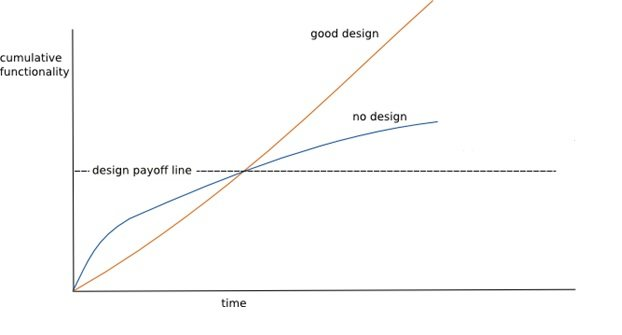
\includegraphics[width=0.7\textwidth]{Chapters/4-Refactoring/images/DesignStaminaHypothesis.jpg}
  \caption{Design Stamina Hypothesis \cite{fowler_refactoring_2018}}
  \label{fig:stamina}
\end{figure}


